\section{Stochastic Block Models}
\label{sec:ch5:sbm}

Let's imagine that you have $100$ students, each of whom can go to one of two possible schools: school one or school two. Your network has $100$ nodes, and each node represents a single student. The edges of this network represent whether a pair of students are friends. Intuitively, if two students go to the same school, the probably have a higher chance of being friends than if they do not go to the same school. If you were to try to characterize this using an ER random network, you would run into a problem: you have no way to capture the impact that school has on friendships. To do this, you need to build upon your $ER_n(p)$ model to make things a little more complicated.

The Stochastic Block Model, or SBM, captures this idea by assigning each of the $n$ nodes in the network to one of $K$ communities, and was first introduced by \cite{Holland1983Jun}. A \textit{community} is a group of nodes within the network which have similar properties. In your example case, the communities would represent the schools that students are able to attend. We use $K$ here to just denote an integer greater than $1$ (for example, in the school example we gave above, $K$ is $2$) for the number of {possible} communities that nodes could be members of. In an SBM, instead of describing all pairs of nodes with a fixed probability like with the ER model, you instead describe properties that hold for edges between {pairs of communities}. In your example, what this means is that if two students go to school one, the probability that they are friends might be different than if the two students went to school two, or if one student went to school one and the other to school two.

\subsection{Defining the SBM random network}
\subsubsection{The community assignment vector assigns nodes in the random network to communities}

To describe an SBM random network, we proceed very similarly to an ER random network, with a twist. An SBM random network has a parameter, $\vec z$, which has a single element for each of the node. We call $\vec z$ the \textit{community assignment vector}, which means that for each node of your random network, $z_i$ tells you which community the node is in. To state this another way, $\vec z$ is a vector where each element $z_i$ can take one of $K$ possible values, where $K$ is the total number of communities in the network. For example, if you had an SBM random network with four nodes in total, and two total communities, each element $z_i$ can be either $1$ or $2$. If the first two nodes were in community $1$, and the second two in community $2$, you would say that $z_1 = 1$, $z_2 = 1$, $z_3 = 2$, and $z_4 = 2$, which means that $\vec z$ looks like:

\begin{align*}
    \vec z &= \begin{bmatrix}1 \\ 1 \\ 2 \\ 2\end{bmatrix}
\end{align*}
\subsubsection{The block matrix defines the edge existence probabilities between communities in the random network}

The other parameter for an SBM random network is called the block matrix, for which we will use the capital letter $B$. If there are $K$ communities in the SBM random network, then $B$ is a $K \times K$ matrix, with one entry for each pair of communities. For instance, if $K$ were two like above, $B$ would be a $2 \times 2$ matrix, and would look like this:
\begin{align*}
    B &= \begin{bmatrix}
        b_{11} & b_{12} \\ b_{21} & b_{22}
    \end{bmatrix}
\end{align*}
Each of the entries of $B$, which we denote as $b_{kl}$ in the above matrix, is a probability of an edge existing between a node in community $k$ and a node in community $l$. 

\subsubsection{Conceptualizing the SBM}

Fortunately, you can also think of this formulation of a random network using coin flips. In your mini example above, if node $1$ is in community $1$ (since $z_1 = 1$) and node $2$ is in community $1$ (since $z_2 = 1$), you have a weighted coin which has a probability $b_{11}$ (the first row, first column of the block matrix above) of landing on heads, and a $1 - b_{11}$ chance of landing on tails. An edge between nodes one and two exists if the weighted coin lands on heads, and does not exist if that weighted coin lands on tails. If you wanted to describe an edge between nodes one and three instead, note that $z_3 = 2$. Therefore, you use the entry $b_{12}$ as the probability of obtaining a heads for the weighted coin you flip this time. In the general case, to use the block matrix to obtain the probability of an edge $(i, j)$ existing between any pair of nodes $i$ and $j$, you will flip a coin with probability $b_{z_i z_j}$, where $z_i$ is the community assignment for the $i^{th}$ node and $z_j$ is the community assignment for the $j^{th}$ node.

If $\mathbf A$ is an SBM random network with $n$ nodes, the community vector $\vec z$, and the block matrix $B$, we say that $\mathbf A$ is an $SBM_n(\vec z, B)$ random network.

\subsection{How do you simulate samples of $SBM_n(\vec z, B)$ random networks?}

The procedure in Algorithm \ref{alg:ch5:sbm} will produce for you a network $A$, which has nodes and edges, where the underlying random network $\mathbf A$ is an $SBM_n(\vec z, B)$ random network.

\begin{algorithm}[h]\caption{Simulating a sample from an $SBM_n(\vec z, B)$ random network}
\label{alg:ch5:sbm}
\SetAlgoLined
\KwData{$n$ a number of nodes\newline $\vec z$ a community assignment vector for each of the $n$ nodes to one of $K$ communities \newline $B$ a probability matrix for each pair of the $K$ communities}
\KwResult{The adjacency matrix of a sample from the random network.}

For each pair of communities $k$ and $l$, obtain a weighted coin (which we will call the $(k,l)$ coin). This coin should have a $b_{kl}$ chance of landing on heads, and a $1 - b_{kl}$ chance of landing on tails.

\For{$i$ in $1$ : $n$} {
    \For{$j > i$} {
        Flip the $(z_i, z_j)$ coin, and if it lands on heads, the corresponding entry $a_{ij}$ in the adjacency matrix is $1$. If it lands on tails, the corresponding entry $a_{ij}$ in the adjacency matrix is $0$.

        Let $a_{ji} = a_{ij}$.
    }
}

\Return{$A$}
\end{algorithm}

We just covered a lot of intuition! This intuition will come in handy later, but let's take a break from the theory by working through an example. Let's use the school example we started above. Say you have $100$ students, and you know that each student goes to one of two possible schools. Remember that you already know the community assignment vector $\vec{z}$ ahead of time. We don't really care too much about the ordering of the students for now, so let's just assume that the first $50$ students all go to the first school, and the second $50$ students all go to the second school. 

\begin{floatingbox}[h]\caption{Though exercise}
Think to yourself what you would expect the node assignment vector and the probability matrix to look like.
\end{floatingbox}

Next, let's plot what the community assignment vector looks like for the network:

\begin{lstlisting}[style=python]
from graphbook_code import plot_vector
import numpy as np

n = 100  # number of students

# z is a column vector of 50 1s followed by 50 2s
# this vector gives the school each of the 100 students are from
z = np.array([1 for i in range(0, n//2)] + [2 for i in range(0, n//2)])
plot_vector(z, title="$\\vec z$, Node Assignment Vector",
            legend_title="School", color="qualitative", 
            ticks=[0.5, 49.5, 99.5], ticklabels=[1, 50, 100],
            ticktitle="Student")
\end{lstlisting}

The community assignment vector is shown in Figure \ref{fig:ch5:sbm}(A). Notice that the first $50$ students are all from school $1$, and the second $50$ students are all from school $2$.

Let's assume that the students from the first school are more friendly than the students from the second school, so we'll say that the probability of two students who both go to the first school being friends is $0.6$, and the probability of two students who both go to school $2$ being friends is $0.4$. Finally, let's assume that if one student goes to the first school and the other student goes to school $2$, that the probability that they are friends is $0.2$. This gives us the ingredients that we need to define the block matrix $B$. 

We can make a block matrix and plot it using the \texttt{heatmap()} utility that you are used to. When working with probabilities or probability matrices, you will usually want to visualize these on a \texttt{[0, 1]} scale, which we can accomplish with the \texttt{vmin, vmax} arguments to our heatmap utility:

\begin{lstlisting}[style=python]
from graphbook_code import heatmap

K = 2  # 2 communities in total
# construct the block matrix B as described above
B = np.array([[0.6, 0.1], 
              [0.1, 0.4]])

ax = heatmap(B, xticklabels=[1, 2], yticklabels=[1,2], vmin=0, 
             vmax=1, annot=True, title="$B$, xtitle="School",
             ytitle="School", title="Block Matrix")
\end{lstlisting}

As you can see in Figure \ref{fig:ch5:sbm}(B), the matrix $B$ is a symmetric block matrix, since your network is undirected. 

\begin{figure}
    \centering
    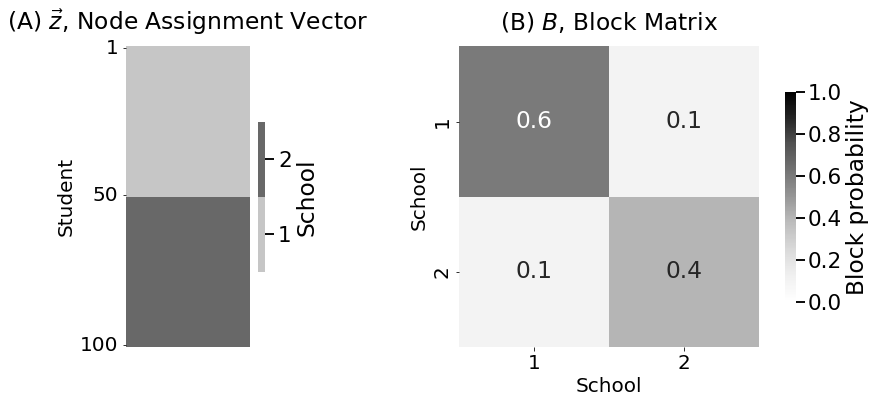
\includegraphics[width=\linewidth]{representations/ch5/Images/sbm.png}
    \caption[Parameters for a stochastic block model]{\textbf{(A)} the community assignment vector for each node (students). \textbf{(B)} the block matrix, which defines the probabilities of a pair nodes (students) from a given community having an edge.}
    \label{fig:ch5:sbm}
\end{figure}

Finally, let's sample and plot a single network from the $SBM_n(\vec z, B)$ with parameters $\vec z$ and $B$:

\begin{lstlisting}[style=python]
from graspologic.simulations import sbm
from graphbook_code import draw_multiplot

# sample a graph from SBM_{100}(tau, B)
A = sbm(n=[n//2, n//2], p=B, directed=False, loops=False)
ys = [1 for i in range(0, 50)] + [2 for i in range(0, 50)]
draw_multiplot(A, labels=ys, title="$SBM_n(z, B)$ Simulation");
\end{lstlisting}

The adjacency matrix is shown in Figure \ref{fig:ch5:sbm_adj}(A).

The above network shows students, ordered by the school they are in (first school and the second school, respectively). As you can see in the network, people from the first school are more connected than people from school $2$. This heatmap can be described as \textit{modular}: it has clear community structure. The connections between people from different schools appear to be a bit {more sparse} (fewer edges) than connections between people from the same school.

When the nodes are ordered by community, we will often refer to ``patches'' (formally, \textit{subnetworks}, from Section \ref{sec:ch4:prop-net:subnetwork}) of the adjacency matrix as \textit{blocks}. The $(k, l)$ block of the adjacency matrix is the block of the adjacency matrix corresponding the the connections between nodes in community $k$ with nodes in community $l$. For instance, the $(1, 1)$ block of the adjacency matrix corresponds to the upper-left block, which is the subnetwork induced by the nodes from community $1$. The $(1,2)$ block of the adjacency matrix corresponds to the upper-right block, which is the subnetwork consisting of nodes in communities $1$ and $2$, but only the edges from nodes in community $1$ to nodes in community $2$. The blocks $(k, k)$ will be referred to as the \textit{on-diagonal} blocks, in that they are the blocks that occur along the diagonal of the adjacency matrix. The blocks $(k, l)$ where $k \neq l$ will be referred to as the \textit{off-diagonal} blocks, in that they are the blocks that do not fall right along the diagonal of the adjacency matrix. Here, the on-diagonal blocks look to have far more connections than the off-diagonal blocks.

In this case, the \textit{modular} structure simply suggests that the different blocks (distinguished by the communities of the different nodes) are readily apparent.


\subsubsection{Modularity is not a pre-requisite for $SBM_n(\vec z, B)$ random networks}
\label{sec:ch5:sbm:modularity}

Something easy to mistake about a sample of an SBM is that the samples will {not always} have the obvious modular structure you can see in Figure \ref{fig:ch5:sbm_adj}(A) when you look at a heatmap. Rather, this modular structure is {only} made obvious because the students are ordered according to the school in which they are in. What do you think will happen if you look at the students in a random order? Do you think that he structure that exists in this network will be obvious?

The answer is: {No!} Let's see what happens when we reorder the nodes from the network into a random order, and pretend you don't know the true community labels ahead of time:

\begin{lstlisting}[style=python]
import numpy as np

# generate a reordering of the n nodes
vtx_perm = np.random.choice(n, size=n, replace=False)

Aperm = A[tuple([vtx_perm])] [:,vtx_perm]
yperm = np.array(ys)[vtx_perm]
heatmap(Aperm, title="Nodes randomly reordered")
\end{lstlisting}

\begin{figure}[h]
    \centering
    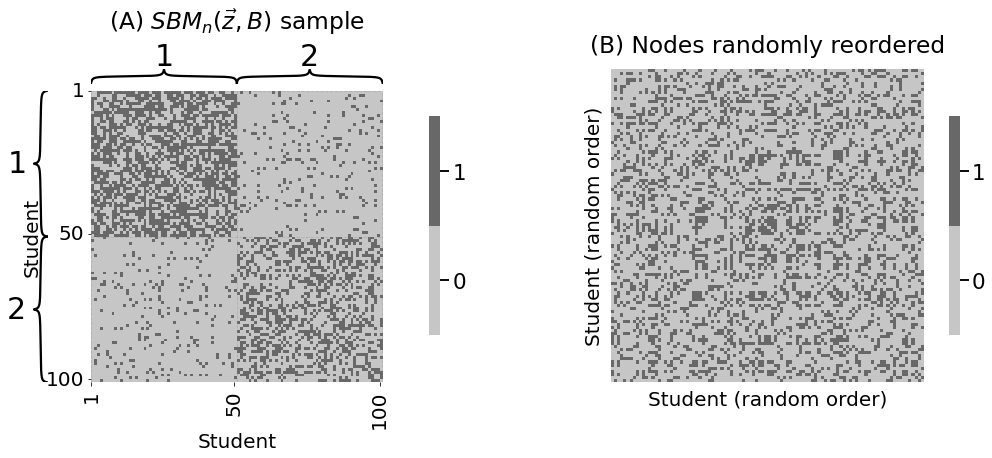
\includegraphics[width=\linewidth]{representations/ch5/Images/sbm_adj.png}
    \caption[Adjacency matrix for SBM with a community ordering of nodes and a random ordering of the nodes]{\textbf{(A)} the adjacency matrix for an $SBM_n(\vec z, B)$ simulation. The parameters are shown in Figure \ref{fig:ch5:sbm}. \textbf{(A)} the same adjacency matrix, but with the nodes randomly reordered.}
    \label{fig:ch5:sbm_adj}
\end{figure}
In Figure \ref{fig:ch5:sbm_adj}(B), the students are {not} organized according to school, because they have been randomly reordered. It becomes pretty tough to figure out whether there are communities just by looking at the adjacency matrix, unless you are looking at a network in which the nodes are {already arranged} in an order which respects the community structure. By an {order that respects the community structure}, we mean that the community assignment vector $\vec z$ is arranged so that all of the nodes in the first community come first, followed by all of the nodes in the second community, followed by all of the nodes in the third community, so on and so forth up to the nodes of the community $K$.

In practice, this means that if you know ahead of time what natural groupings of the nodes might be (such as knowing which school each student goes to) by way of your node attributes, you can visualize your data according to that grouping. This property is covered more in depth by \cite{Abbe2017Mar}. If you don't know anything about natural groupings of nodes, however, you are left with the problem of {estimating community structure}. A later method, called the {spectral embedding} in {numref}`ch6:spectral`, will be paired with clustering techniques to allow you to estimate node assignment vectors. 

We'll conclude off this section by showing that the previous random network model you saw, the ER random networks, are special cases of SBM random networks. These properties will become useful as you build more and more complex random network models, because when you develop techniques for more complex random network models in later chapters, they will extend directly to any network model which is a special case of that random network model.

\subsection{ER random networks are special cases of SBM random networks}

Let's imagine that you have a random network $\mathbf A$ which is $ER_n(p)$. Could you take this random network and turn it into an SBM? More specifically, does there exist an SBM such that the edge-existence probabilities are the same as the $ER_n(p)$ random network, for {every} edge in the network?

The answer is {always} a yes! This is extremely easy. Take the number of edge communities for the corresponding SBM to be $1$, and assign every node to the first community. Next, take the block matrix to have a single entry, $b_{11} = p$. And you are done! $\mathbf A$ is also an $SBM_n(\vec z, B)$ random network, where $\vec z$ is a vector of ones, and $B$ is a $1 \times 1$ matrix (really, just a scalar) whose only entry is $p$.

We are finished! To see that the edge-existence probabilities are the same, you'll back up to your coin flips. In the ER random network, you performed a coin flip for each edge $\mathbf a_{ij}$ with a coin that landed on heads with probability $p$. In the SBM random network, you performed a coin flip for each edge $\mathbf a_{ij}$ with a coin that landed on heads with probability $b_{z_i z_j}$. Here, there is only one possible value that $z_i$ or $z_j$ could take; they both must be one, since there is only one community. Therefore you flip a coin that lands on heads with probabaility $b_{11}$. But when you built the block matrix, we said that $b_{11}$ was just $p$, so the coin flip is occurring with a coin that lands on heads with probability $p$. This is obviously the same procedure you took with the ER random network at all possible edges, so the edge-existence probabilities are all identical. Therefore, the $ER_n(p)$ random network is also an $SBM_n([1, 1, ..., 1], B = [p])$ random network.

\subsection{Read on for more}

If you want a deeper level of technical depth on Stochastic Block Models, please see Appendix \ref{app:ch12:sbms}.


\newpage